% 
% Annual Cognitive Science Conference
% Sample LaTeX Paper -- Proceedings Format
% 

% Original : Ashwin Ram (ashwin@cc.gatech.edu)       04/01/1994
% Modified : Johanna Moore (jmoore@cs.pitt.edu)      03/17/1995
% Modified : David Noelle (noelle@ucsd.edu)          03/15/1996
% Modified : Pat Langley (langley@cs.stanford.edu)   01/26/1997
% Latex2e corrections by Ramin Charles Nakisa        01/28/1997 
% Modified : Tina Eliassi-Rad (eliassi@cs.wisc.edu)  01/31/1998
% Modified : Trisha Yannuzzi (trisha@ircs.upenn.edu) 12/28/1999 (in process)
% Modified : Mary Ellen Foster (M.E.Foster@ed.ac.uk) 12/11/2000
% Modified : Ken Forbus                              01/23/2004
% Modified : Eli M. Silk (esilk@pitt.edu)            05/24/2005
% Modified : Niels Taatgen (taatgen@cmu.edu)         10/24/2006
% Modified : David Noelle (dnoelle@ucmerced.edu)     11/19/2014
% Modified : Roger Levy (rplevy@mit.edu)     12/31/2018



%% Change "letterpaper" in the following line to "a4paper" if you must.

\documentclass[10pt,letterpaper]{article}

\usepackage{cogsci}

% \cogscifinalcopy % Uncomment this line for the final submission 


\usepackage{pslatex}
\usepackage{apacite}
\usepackage{float} % Roger Levy added this and changed figure/table
                   % placement to [H] for conformity to Word template,
                   % though floating tables and figures to top is
                   % still generally recommended!

%\usepackage[none]{hyphenat} % Sometimes it can be useful to turn off
%hyphenation for purposes such as spell checking of the resulting
%PDF.  Uncomment this block to turn off hyphenation.


%\setlength\titlebox{4.5cm}
% You can expand the titlebox if you need extra space
% to show all the authors. Please do not make the titlebox
% smaller than 4.5cm (the original size).
%%If you do, we reserve the right to require you to change it back in
%%the camera-ready version, which could interfere with the timely
%%appearance of your paper in the Proceedings.

% erikb new packages
\usepackage{graphicx}
\usepackage{color}
\newcommand{\eb}[1]{{\color{blue}{\bf\sf [EB: #1]}}}



\title{How do people incorporate advice from\\ artificial agents when making physical judgments?}
 

\author{
  {
  % Erik
  \large \bf Erik Brockbank* (ebrockbank@ucsd.edu)} \\
  UCSD Department of Psychology, 9500 Gilman Drive \\
  La Jolla, CA 92093 USA
  % Haoliang
  \AND {\large \bf Haoliang Wang* (haw027@ucsd.edu)} \\
  UCSD Department of Psychology, 9500 Gilman Drive \\
  La Jolla, CA 92093 USA
  % Justin
  \AND {\large \bf Justin Yang (juy003@ucsd.edu)} \\
  UCSD Department of Psychology, 9500 Gilman Drive \\
  La Jolla, CA 92093 USA
  % Suvir
  \AND {\large \bf Suvir Mirchandani (suvir@cs.stanford.edu)} \\
  Stanford Department of Computer Science, 353 Jane Stanford Way \\
  Stanford, CA 94305 USA \\
  % Erdem
  \AND {\large \bf Erdem B{\i}y{\i}k (ebiyik@stanford.edu)} \\
  Stanford Department of Electrical Engineering, 353 Jane Stanford Way \\
  Stanford, CA 94305 USA \\
  % Dorsa
  \AND {\large \bf Dorsa Sadigh (dorsa@cs.stanford.edu)} \\
  Stanford Department of Computer Science, 353 Jane Stanford Way \\
  Stanford, CA 94305 USA \\
  % Judy
  \AND {\large \bf Judith Fan (jefan@ucsd.edu)} \\
  UCSD Department of Psychology, 9500 Gilman Drive \\
  La Jolla, CA 92093 USA \\
}


\begin{document}

\maketitle


\begin{abstract}
How do people build up trust with artificial agents? Here, we study a key component of interpersonal trust: people's ability to evaluate the \textit{competence} of another agent across repeated interactions. Prior work has largely focused on appraisal of simple, static skills; in contrast, we probe competence evaluations in a rich setting with agents that learn over time. Participants played a video game involving physical reasoning paired with one of four artificial agents that suggested moves each round. We measure participants' decisions to accept or revise their partner's suggestions to understand how people evaluated their partner's ability. Overall, participants collaborated successfully with their agent partners; however, when revising their partner's suggestions, people made sophisticated inferences about the competence of their partner from prior behavior. Results provide a quantitative measure of how people integrate a partner's competence into their own decisions and may help facilitate better coordination between humans and artificial agents.

\textbf{Keywords:} 
trust; social inference; artificial agents; competence; learning 
\end{abstract}



\section{Introduction}

\textit{How do people build up trust across repeated interactions?} This question has motivated research from diverse areas of cognitive science spanning social psychology \cite{simpson2007psychological, deutsch1973resolution} as well as game theory and economics \cite{camerer1988experimental, berg1995trust}. As artificial intelligence agents become increasingly ubiquitous in our everyday lives, the question of how to build up trust with them has also gained prominence in robotics and human-computer interaction (HCI) \cite{soh2020multi, chen2020trust}. 
In autonomous driving settings for instance, people routinely make decisions about how much to trust an artificial driving agent. And in many industrial domains, people work closely with automated agents, sometimes for high stakes tasks. The emergence of trust in our interactions with artificial agents involves a range of complex social inferences, such as recognizing that they share our goals or utilities to begin with \cite{serrino2019finding}. However, one of the central features of human collaboration with artificial agents is that we trust them to be \textit{competent} across a range of task settings. Indeed, greater levels of trust may simply correspond to a belief that the agents are competent in a wider range of settings; for example, trust in an autonomous vehicle may in large part reflect a belief that it can handle a suitably broad array of driving challenges.

How then do people assess another agent's competence over repeated interactions? Prior work in developmental psychology suggests that inferences about another person's competence emerge early in development and draw on a rich set of abstractions about task difficulty and human behavior \cite{gweon2021inferential, leonard2019better}. As adults, this ability continues to develop, allowing us to make complex inferences about other people which draw on rich internal models \cite{velez2019integrating, velez2021learning}, meta-cognitive skills \cite{pescetelli2021role}, and expectations \cite{leong2018unrealistic, chang2010seeing}. Recent work in robotics and HCI suggests that when determining a robot or artificial agent's competence, people may rely on similar cognitive processes, leveraging abstractions about both the agent---e.g., their risk aversion \cite{xie2019robot}---and the environment, such as how much the agent's ability will generalize across tasks \cite{soh2020multi}. 

Despite this convergence of findings across psychology and artificial intelligence, there remain significant challenges in characterizing how people assess the competence of another agent. For one, real-world judgments of competence are often nebulous. How good is somebody at baking or predicting the stock market or writing academic papers? Second, in many complex settings, people's judgments of another agent's competence rely in large part on that agent's ability to \textit{learn} in the task environment. The current work builds on prior results by addressing both of these aspects of people's competence evaluations. First, unlike prior work on advice taking that has focused on judgments about abstract variables, e.g., change in stock market prices \cite{leong2018unrealistic} or the outcome of a card flip \cite{velez2019integrating}, here we explore how people incorporate input from an artificial agent when predicting concrete physical events. Second, rather than isolating competence judgments about static agents \cite{chen2020trust}, the current experiment probes people's ability to detect another agent's \textit{learning} over time. A better understanding of how an agent's learning impacts competence judgments in a rich physical domain may support a broader conceptualization of how people reason about the abilities of others, and how this reasoning impacts their subsequent decisions to trust them in a range of everyday settings.



% FIGURE: Stimuli
\begin{figure*}[hbtp]
% \centering
\vspace{-8mm}
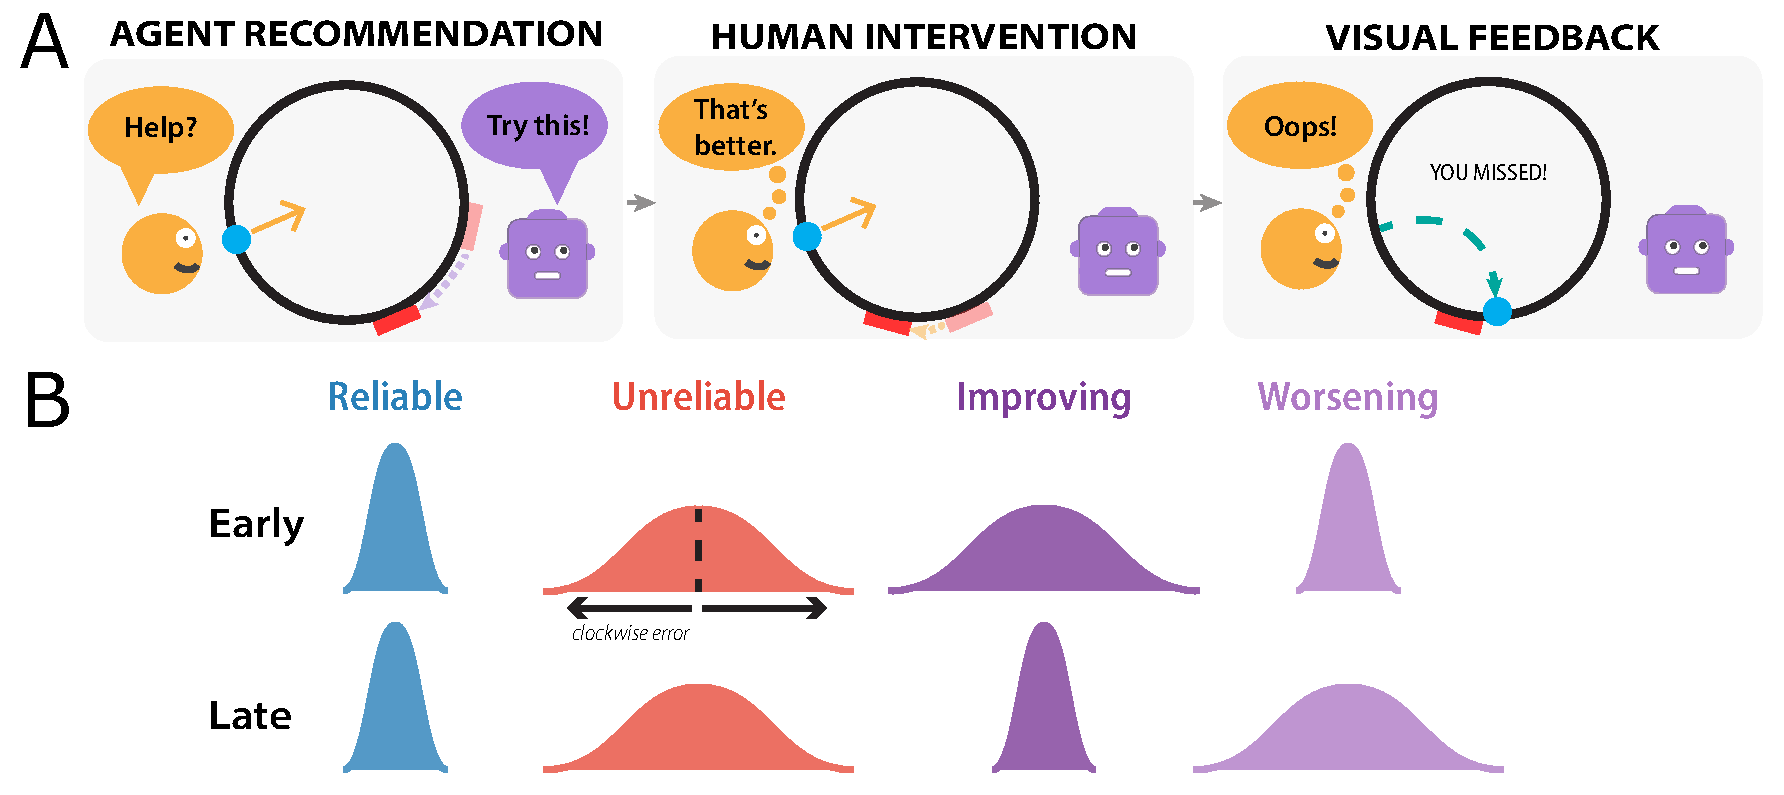
\includegraphics[width=\textwidth]{img/expt_overview.pdf} 
\vspace{-4mm}
\caption{Task and Experimental Design. (A) Participants worked with an artificial agent partner to catch a ball launched from the edge of a circle. Their partner began by suggesting a paddle location which participants could either accept or modify. (B) The agents chose suggested paddle locations from a distribution around the ball's true landing position. The variance of this distribution determined how reliable the agent's suggestions were. Participants were assigned to one of four conditions that varied the reliability of the agent's paddle suggestions over the course of the experiment.} 
\label{fig:stimuli}
\end{figure*}



Here, we investigate people's ability to collaborate with a dynamic artificial agent in a challenging physics-based video game. Participants were tasked with catching a ball launched from different locations around a circle by placing a paddle where the ball would land. Each round, they were given a suggestion from their agent partner about where to place the paddle to catch the ball. Building on prior work, we use people's decisions about whether to accept or modify their partner's suggestions to probe people's judgments of their partner's competence \cite{xie2019robot, chen2020trust}. Critically, people's agent partners varied in their true competence and improvement over time. We first ask how much people's behavior in the game draws on their own physical judgments versus the suggestions of their partner and how this varies based on their partner's competence. Next, we ask whether people's intervention decisions reflect ongoing assessments of their partner's ability rather than trial-specific context. Our results contain three key findings. First, rather than relying exclusively on their own physical judgments or the advice of their partner, people integrated both sources of information in their interventions. Moreover, the degree to which they incorporated their partner's input was predicted by how reliable the agent had been in the past, not just the quality of its current advice. Finally, when the quality of an agent's advice changes over time, people adapted to these changes but their initial experience with the agent exerted a disproportionate influence on how much they trusted the agent's recommendations. Broadly, simple collaborative decisions involve rich, abstract inferences about others based on their past behavior.
 

\section{Experiment}

\subsection{Participants}

256 adults recruited from Prolific completed the task online. Data from 12 participants were excluded from subsequent analyses due to technical issues encountered during the experiment, resulting in 244 participants with complete data (average age: 33.8 years, $SD$ = 11.3; 127 male, 103 female, 13 non-binary; educational background distributed across high school, 4-year college, and graduate degrees). The experiment lasted approximately 25 minutes and participants were paid \$14/hr based on this expected completion time. 


\subsection{Stimuli}

In this experiment, participants tried to catch a virtual ball launched from a point on a circle using a rectangular paddle positioned along the outside of the circle (see Figure \ref{fig:stimuli}).\footnotemark{} 
Participants worked together with an artificial agent ``partner'' who was trying to help them on the task. In each round, the partner suggested a paddle location based on the ball's starting position; participants could either accept this suggestion or adjust the paddle themselves before launching the ball.

\footnotetext{All code used to run the experiment, as well as code used in analyses below, can be found at: MASKED FOR ANONYMOUS REVIEW.}

Participants were assigned to one of four conditions that manipulated the quality of their partner's suggested paddle locations: an \textit{unreliable} partner, a \textit{reliable} partner, an \textit{improving} partner, and a \textit{worsening} partner. The agent's
suggested paddle location in each trial was an angle $x$ sampled from a von Mises distribution (an approximation of a normal distribution defined over angles around a circle) with mean $\mu$ equal to the ball's final landing angle $\rho$, and variance $\sigma^2$ set based on the agent's competence level for that condition. The \textit{reliable} agent had a low $\sigma^2$ value of roughly 10 degrees, meaning that the sampled paddle location was almost always close to the ball's true landing location. In contrast, the \textit{unreliable} agent sampled its paddle locations from a high variance distribution with $\sigma^2 \approx 48$ degrees, meaning that while suggestions on some trials were accurate, many were not. The high and low competence $\sigma^2$ values were chosen to give the agents expected success rates of around $80\%$ and $20\%$, respectively. Meanwhile, the \textit{improving} agent began with a $\sigma^2$ value equal to the \textit{unreliable} agent's high $\sigma^2$ value, but every 12 trials the variance decreased by a fixed amount so that during the final 12 trials, it had a $\sigma^2$ equal to the \textit{reliable} agent. The \textit{worsening} agent was symmetrical but in the opposite direction.

The task was composed of 96 trials divided into eight blocks of 12. These ``blocks'' were not visible to participants; in each block of trials, the ball appeared at a location sampled from each of the 12 hours on a clock face with some jitter so that participants would not rely on regularity in ball launch locations. The trials were randomized in each block so there was no structured pattern from one launch location to the next. The blocks were also used to update the performance of the \textit{improving} and \textit{worsening} agents described above; within each block, they had a stable success rate that was better (\textit{improving}) or worse (\textit{worsening}) than the previous block. The ball's launching locations were pre-computed to allow for simulations that calculated the ball's final landing location; they were therefore the same for every participant. The agents' suggested paddle locations were sampled each trial, allowing them to vary across participants. 

During each block, a randomly chosen trial was designated as a \textit{critical trial} to measure differences in how much people trusted their partner across conditions (participants were not informed of this); rather than sampling the agent's recommendation as described above, the suggested paddle location on critical trials was chosen to have a fixed distance from the ball's landing location. This distance (0.28 radians, roughly 16 degrees) was chosen to ensure that the agent's suggestion would not catch the ball but would be close to where it landed. Each participant saw eight critical trials over the course of the experiment. This enabled comparison of intervention behavior with partners that differed in overall accuracy when the error of their paddle suggestion in these trials was the same. 


\subsection{Procedure}

Each trial began with participants' agent partner suggesting a paddle location that would catch the ball; the paddle was shown moving around the circle and a small animation on the right showed the agent ``thinking.'' Once the agent had moved the paddle to its suggested location, participants were given the opportunity to either adjust the paddle with the arrow keys or keep their partner's suggestion. If participants adjusted the paddle, the agent's original recommendation was indicated with a gray outline so participants would be able to see how close the ball landed to the partner's suggestion. When participants settled on a paddle location, they launched the ball with the spacebar. The ball's path was animated and participants were shown a message indicating whether they had successfully caught it before proceeding to the next trial. 

After completing all 96 trials, participants were given a post-experiment questionnaire. First, a series of demographic questions prompted them for their age, gender identity (optional), level of education, and two covariates which we did not analyze here: prior academic physics courses and prior experience with video games. Next, they were asked several questions about their decisions during the experiment. On a slider scale ranging from $0-100\%$, participants indicated how often they thought they had intervened on the previous trials and how often they would expect to intervene if they were to play another 96 rounds with this same partner. Finally, they were asked to indicate on a five-point rating scale how much they trusted the agent to catch the ball and how they decided whether to intervene on a given trial (two additional questions asked how much effort they had put into the task and whether they had experienced technical difficulties).


\section{Results}

\subsection{People combine information sources to make intervention decisions}

To understand how participants chose whether to intervene or trust their partner, we compare three possible accounts of their decision making. First, it may be that people were entirely trusting of their agent partner, regardless of its competence. On this view, participants' own physical intuitions would have played no role in their decision making. A second account takes the opposite perspective; people may have ignored their partner's suggestions, simply choosing the best paddle position each round (i.e., if the agent's suggestion was accurate, people would accept it and if not, they would intervene to correct it). Finally, a third account is that people's behavior was somewhere in the middle of these two. Rather than consistently following their partner's suggestion or unilaterally seeking the optimal paddle position each round, people may have relied on a combination of their own physical intuitions and information provided by their partner's suggestion to decide where to place the paddle. We consider each of these options below; our results suggest that participants integrated intuitive physical judgments with their partner's guidance and that \textit{how much} they incorporated their partner's suggestion was calibrated to the their partner's ability.


\subsubsection{Participants intervened to improve accuracy.} 

We start by considering the first hypothesis above, that people merely acted in accordance with their partner's suggestions. If this were true, we would expect intervention rates to be low and overall performance to closely match the ability of the agents in each condition. Figure \ref{fig:interventions} (top) shows the average of each subject's intervention rate (the percent of trials in which they modified the agent's original suggestion) in each trial block. Notably, intervention rates were high in all conditions; even with the \textit{reliable} agent, whose suggestions would catch the ball on approximately 80\% of trials, participants consistently intervened over 50\% of the time. Alongside the high overall intervention rates, intervention behavior between conditions reflected the different competence levels of each agent and showed a sensitivity to the changing accuracy of the \textit{improving} and \textit{worsening} agents. Thus, far from merely trusting their partner's suggestions, participants took an active role in calibrating their interventions to their partner's ability.

But how successful were these interventions? We calculated the average root mean squared error (RMSE) of each participant's paddle location relative to the ball's final landing location and compared this to the average RMSE of the agent recommendations to assess whether participants' interventions improved accuracy. Average participant RMSE was significantly lower than their partner's suggestions in the conditions where bot suggestions had large error (\textit{improving}: $t(64) = -8.36$; \textit{worsening}: $t(54) = -17.92$; \textit{unreliable}: $t(66) = -26.71$, all $p$s $<0.001$), but not in the \textit{reliable} condition where bot suggestions were already close to the ball's landing location ($t(56) = 0.59$, $p = 0.56$). Participants were able to master the task by intervening in a way that was calibrated to their partner's ability. Further, it rules out one concern with the current results, namely that participants' decision to follow their partner's guidance was a result of finding the task difficult and having little confidence in their own interventions. Given that participants were able to perform better than they would have if they had simply followed their partner's recommendations, it seems unlikely that their intervention decisions reflected challenges with the task.



\begin{figure}[t]
\begin{center}
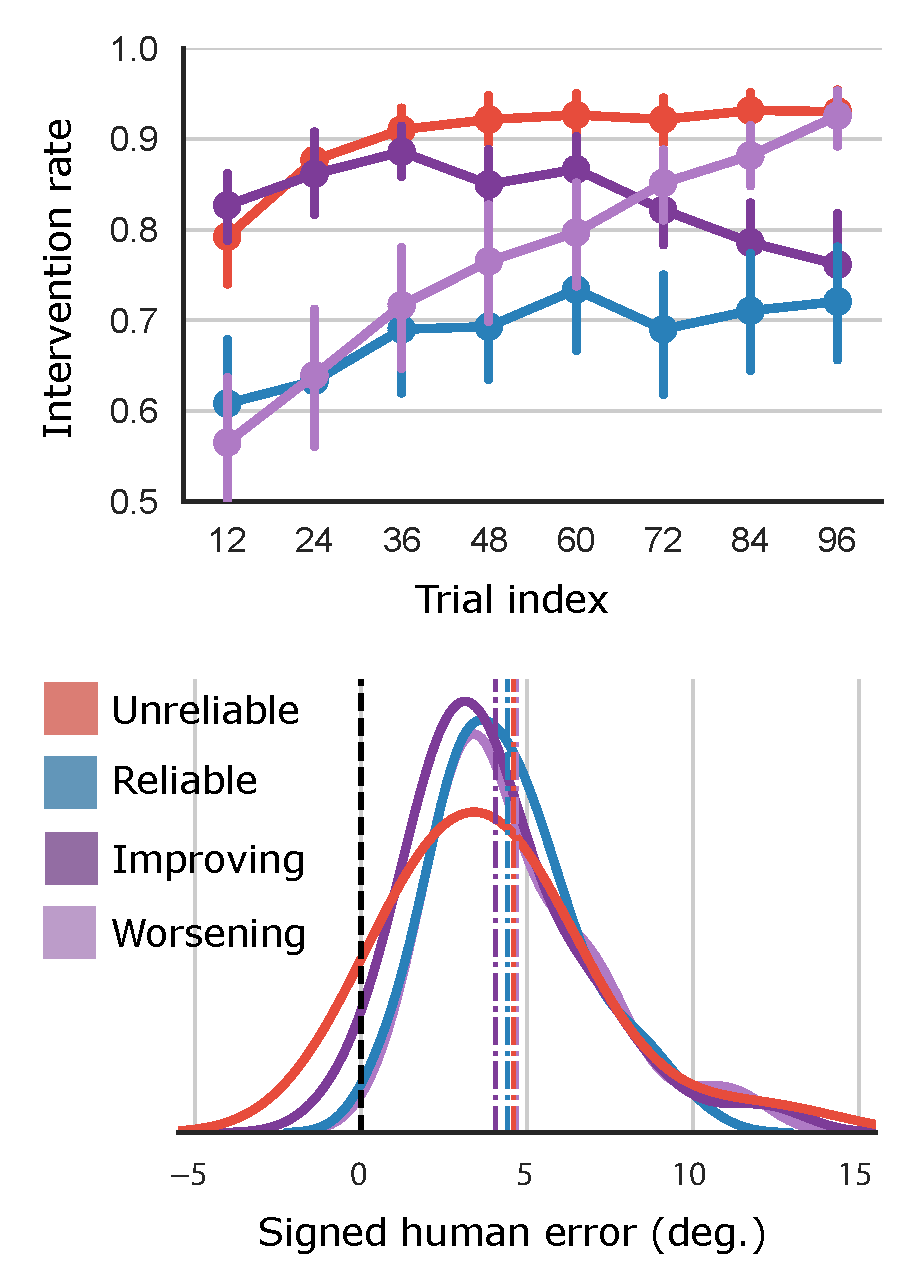
\includegraphics[width=0.9\linewidth]{img/error_interventions_combined.pdf}
\end{center}
\caption{
Top: Average of each participant's paddle intervention rates by trial block. 
Bottom: Distribution of participants' average trial error in each condition, with positive values indicating responses whose error was in the same direction as the agent's suggestion and negative values indicating the opposite. The black dashed line indicates the true landing location of the ball. Colored vertical lines indicate means in each condition. Curves are based on kernel density estimation.}
\label{fig:interventions}
\end{figure}



\subsubsection{Intervention decisions incorporated agent suggestions.}

In light of the high intervention rates across conditions, one account of people's behavior is that they simply relied on their own intuitive physics to respond. Critically, on this view, their partner's ability would have been essentially irrelevant. In other words, we would expect the agent's suggestion to have no impact on people's behavior, e.g., minimal adjustments in the \textit{reliable} condition would simply reflect the fact that on most trials, little adjustment was needed. 

To test this possibility, we examine the distribution of participants' \textit{errors} on each trial relative to both the ball's final landing location and their partner's suggestion. Intuitively, if people were essentially ignoring their partner, we would expect their errors to be roughly normally distributed around the ball's true landing location, just as often to one side as the other, regardless of the agent's paddle suggestion. On the other hand, insofar as people incorporated their partner's suggestion into their decision about where to place the paddle, we might expect the agent's suggested paddle location to have an attractive or repellent effect on participants. Figure \ref{fig:interventions} (bottom) shows the distributions of participants' average error in each condition. Critically, these distributions are signed relative to the ball's landing location and the agent's paddle suggestion, so an average error of 0 (degrees) represents a perfectly accurate paddle placement, while error greater than 0 represents participants placing the paddle away from the ideal catching location \textit{in the direction of the agent's suggestion}. Meanwhile, error less than 0 represents participants placing the paddle away from the ideal location \textit{in the opposite direction of the agent's suggestion}. The dashed lines in Figure \ref{fig:interventions} (bottom) show the average signed error in each condition. Participants' error was significantly greater than $0$ in all four conditions, reflecting a stable bias toward their partner's recommended paddle locations (\textit{reliable}: $t(56) = 15.70$; \textit{improving}: $t(64) = 12.34$; \textit{worsening}: $t(54) = 14.20$; \textit{unreliable}: $t(66) = 8.13$, all $p$s $< 0.001$). This suggests that people's decisions about where to place the paddle were not merely an effort to find the best location independent of their partner's advice; rather, they showed a systematic anchoring towards the agent's recommendation.

Taken together, the results in Figure \ref{fig:interventions} suggest that people's decisions about where to place the paddle integrated multiple sources of information. They did not merely trust their partner regardless of its competence, nor did they simply choose the best move each round without consideration for their partner's recommendation. However, the agent's paddle suggestion on a given trial is not the only source of information that might help participants decide where to ultimately place the paddle. Rather, across repeated interactions, agents in each condition offer evidence of their underlying \textit{competence} through the accuracy of their paddle suggestions. Participants can use this information to calibrate \textit{how much} their final paddle locations should be influenced by their partner. 


\subsection{People relied on past performance to guide interventions}

Since agent partners varied across conditions in how helpful their paddle suggestions were, we hypothesize that participants incorporated this information into their decisions about how closely to follow their partner's suggestions. To do this, participants would have had to maintain an estimate of the overall competence of their partner across repeated trials which could then serve as the basis for deciding how much to be swayed by their partner's suggestions. 

To test this hypothesis, we compare intervention behavior on the eight \textit{critical trials} that each participant completed. If people's responses were merely a result of combining their own estimate of the ball's final location with a consistent offset towards their partner's suggestion, we should not see any difference in intervention behavior on these trials, since the agent's error on critical trials was held constant. However, if people's behavior reflected a judgment about the quality of their partner's advice from previous trials, we might expect their intervention decisions to differ across conditions in line with the underlying differences in agent accuracy. Figure \ref{fig:critical_trials} (top) shows average intervention rates on critical trials. We fit a generalized linear mixed effects model with a binomial link function to participants' intervention behavior (binary) on critical trials; we find that a fixed effect of condition produces a significantly better fit than random intercepts for each participant alone ($\chi^2(3) = 17.8$, $p < 0.001$). Consistent with the pattern observed in Figure \ref{fig:critical_trials} (top), estimated marginal means were significantly different between \textit{unreliable} and \textit{reliable} conditions ($p = 0.01$), as well as \textit{improving} and \textit{reliable} ($p = 0.003$) and \textit{improving} and \textit{worsening} ($p = 0.02$).

The previous results suggest that people's decisions about whether to intervene on critical trials were influenced by their partner's prior accuracy. People displayed a similar pattern in their intervention \textit{magnitudes} on critical trials in which they did intervene (Figure \ref{fig:critical_trials}, bottom). While those paired with an \textit{unreliable} or \textit{improving} partner adjusted the paddle by an amount close to the optimal level, participants whose partner was very accurate (\textit{reliable}) or started out highly accurate (\textit{worsening}) made smaller adjustments on critical trials. As above, a linear mixed effects model predicting intervention distance (on critical trials where participants intervened) as a function of condition performed significantly better than a baseline model which included only random effects of subject ($\chi^2(3) = 28.3$, $p < 0.001$). Estimated marginal means were significantly different across \textit{unreliable} and \textit{reliable} agents ($p < 0.001$), \textit{unreliable} and \textit{worsening} ($p = 0.005$), and \textit{improving} and \textit{reliable} ($p < 0.001$). Thus, a complete account of reasoning on this task suggests that people maintain an underlying assessment of their partner's competence over time and calibrate their decisions about whether to intervene and how much based on this assessment. Further, the significant difference in intervention rates and magnitudes across the \textit{improving} and \textit{worsening} conditions suggests that this appraisal of their partner's ability was not balanced over the experiment; people accorded more weight to their \textit{initial} experience when estimating their partner's competence.



% FIGURE: Critical trials
\begin{figure}[h]
\begin{center}
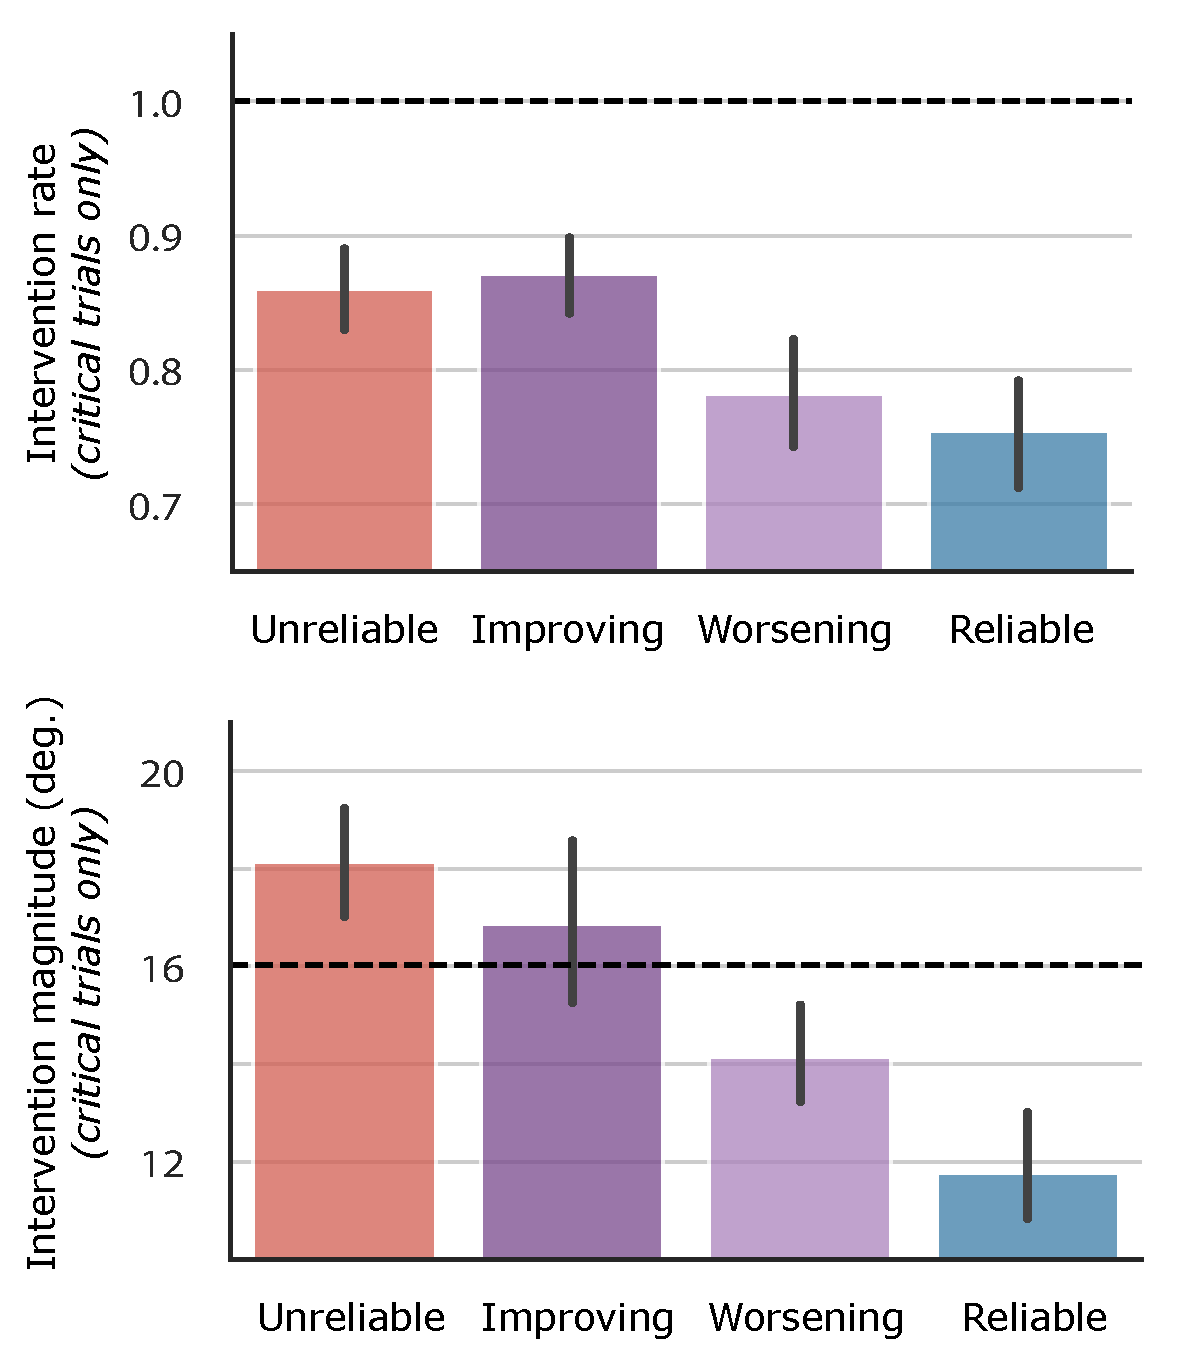
\includegraphics[width=0.9\linewidth]{img/critical_trial_intervention_summary_vert.pdf}
\end{center}
\caption{Intervention behavior on \textit{critical trials}. 
Top: average proportion of critical trials on which participants chose to intervene. The dashed line indicates optimal behavior (critical trials always required intervention to catch the ball). 
Bottom: average distance participants intervened on critical trials in which they chose to intervene. The dashed line indicates the optimal intervention distance on these trials.} 
\label{fig:critical_trials}
\end{figure}



\subsection{Past performance and future expectations}

So far, we have found evidence that participants' decisions about when to intervene with their partner, and how much, rely on an ongoing estimate of their partner's overall competence. \textit{But how do people generate this estimate?} Our previous results indicate that people do not simply average their partner's performance over the most recent trials; instead, first impressions seem to matter more. To better understand the \textit{basis} for participants' judgments of their partner's competence, we examine responses on the post-experiment survey. First, participants' estimates of how often they had intervened in the experimental trials were significantly correlated with their true intervention rates ($r = 0.63$, $p < 0.001$), though participants exhibited a tendency to underestimate intervention rates overall, $t(243) = 4.19$, $p < 0.001$. Thus, people's decisions about whether to intervene on a given trial may have reflected a fairly accurate accounting of past experience. 

But did this enable a calibrated sense of their partner's competence? Figure \ref{fig:survey} shows the estimated intervention rates from experimental trials paired with participants' responses indicating how much they would \textit{expect} to intervene if they played 96 more rounds with the same partner. The difference in these values across conditions provides some indication of how accurately participants formed future expectations about their partner based on past performance. Responses suggest that people's ability to explicitly forecast their partner's future behavior was limited. In a 4 (between-subjects condition: \textit{reliable}, \textit{unreliable}, \textit{improving}, \textit{worsening}) by 2 (within-subjects rating type: \textit{reported}, \textit{expected}) repeated measures ANOVA of the intervention rates shown in Figure \ref{fig:survey}, differences between conditions were significant ($F(3, 240) = 17.16$, $p < 0.001$) and the interaction between condition and rating type was significant ($F(3, 1) = 6.77$, $p < 0.001$). However, in follow-up paired $t$-tests, participants in the \textit{worsening} condition showed a significant difference between past and expected future intervention rates implying some degree of forecasting ($t(54) = -4.80$, $p < 0.001$), but participants in the \textit{improving} condition did not ($t(64) = 0.38$, $p = 0.71$). Forecasted intervention rates remained stable for the \textit{unreliable} and \textit{reliable} agents, as we might expect (\textit{unreliable}: $t(66) = -0.10$, $p = 0.92$; \textit{reliable}: $t(56) = 1.58$, $p = 0.12$). 
Critically, these forecasts reflect participants' underlying trust in their partner. Predicted future intervention rates ($0-100\%$) were significantly negatively correlated with responses on a five-point rating scale question asking how much participants trusted their partner to catch the ball on a given trial (\textit{Not at all}, \textit{Slightly}, \textit{Moderately}, \textit{Very}, \textit{Extremely}), $r = -0.51$, $p < 0.001$. This highlights the potential role of expectations about future behavior in our trust in others.



% FIGURE: post-survey
\begin{figure}[h]
\begin{center}
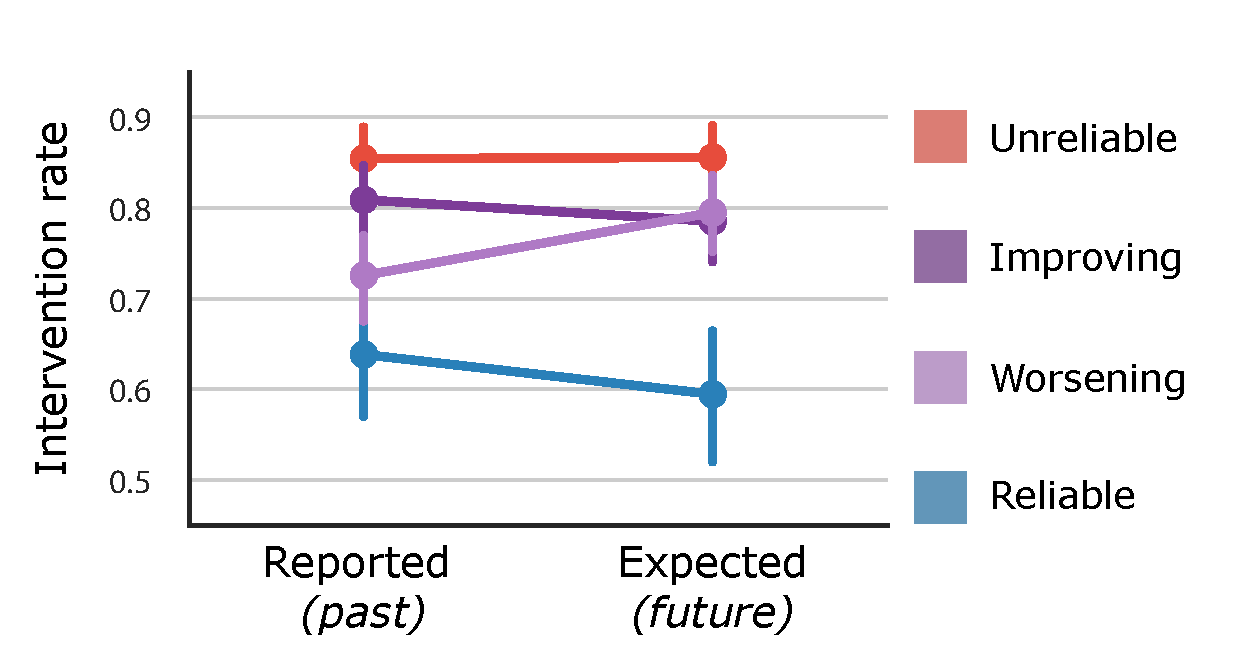
\includegraphics[width=0.9\linewidth]{img/survey_intervention_expectations_clean.pdf}
\end{center}
\caption{Participant estimates of how much they intervened with each agent compared to how much they would expect to intervene in future rounds with the same partner. Results of the post-experiment questionnaire suggest that people form expectations of their partner's future performance based on attributions of the agent's competence.} 
\label{fig:survey}
\end{figure}



\section{Discussion}

In this study, we address the question of how people evaluate an artificial agent's \textit{competence} in a novel setting, a key underpinning of forming trust relationships. Participants played a video game in which they positioned a paddle around the outside of a circle to catch a ball launched from different points around the circle. Participants were paired with an artificial agent who suggested paddle locations on each trial and participants then chose whether to accept or modify their partner's suggestion. Critically, the agents varied in the accuracy of their recommendations, allowing us to explore how differences in competence impacted people's decision to trust their partner. Specifically, we probe people's sensitivity to changes in their partner's ability across repeated interactions in a setting that draws on rich human physical intuitions. Our results contain several key findings. First, we show that participants' decisions in this task involve a combination of their own physical judgments and the recommendations of their partner, rather than exclusively trusting their partner's suggestions or choosing the best move without regard for their partner. In other words, people integrate cues from both their own and their partner's reasoning. Second, we show that this process of integrating information from their partner extends beyond a mere bias towards their partner's estimate; instead, people calibrate \textit{how much to defer to their partner} based on the prior reliability of their partner's suggestions. In other words, their behavior is informed by an ongoing estimate of their partner's competence. We further show that this estimate is not static but rather sensitive to changes in their partner's competence over time. However, this responsiveness to changes in their partner's ability was intriguingly asymmetrical for improving and worsening partners; participants placed significantly more weight on initial experience than recent behavior. In this way, our findings make headway towards a better understanding of the behavioral underpinnings of trust in artificial agents across repeated interactions. 

The current results raise a number of questions about trust and evaluations of competence in others that merit further investigation. First, how nuanced is our perception of another agent's \textit{learning}? While the current work probes this with agents whose suggestions become steadily more reliable, there are a number of ways in which we judge another person or agent's learning over time. For example, future work should explore our ability to decompose a task into different skills and interpret an agent's errors in light of these skills. Second, while the current experiment focuses on a single task domain, a key component of the trust we place in others is the degree to which we believe their competence \textit{generalizes} to new settings. Physical tasks such as the one in our experiment offer a rich opportunity to explore questions of transfer and generalization. By providing a more thorough account of the ways we judge competence from the behavior of others, the current work can inform future efforts aimed at building more trusting relationships and fostering better collaboration between humans and learning agents.




% \section{Acknowledgments}
% In the \textbf{initial submission}, please \textbf{do not include acknowledgements}, to preserve anonymity. 
% In the \textbf{final submission}, place acknowledgments (including funding information) in a section \textbf{at the end of the paper}.





\bibliographystyle{apacite}
\setlength{\bibleftmargin}{.125in}
\setlength{\bibindent}{-\bibleftmargin}
\typeout{} % erikb for some reason this line is necessary...
\bibliography{references}


\end{document}
